\documentclass[11pt,a4j,uplatex]{jsarticle}
\usepackage{ascmac}
\usepackage{amsmath,amssymb}
\usepackage[dvipdfmx]{graphicx}
\usepackage{upgreek}%\upGreek
\usepackage{cases}%連立方程式
\usepackage{bm}%ベクトル表記\bm{A}
\usepackage{bigdelim,multirow}


\newsavebox{\circlebox}
\savebox{\circlebox}{\fontencoding{OMS}\selectfont\Large\char13}
\newlength{\circleboxwdht}
\newcommand{\centercircle}[1]{%
  \setlength{\circleboxwdht}{\wd\circlebox}%
  \addtolength{\circleboxwdht}{\dp\circlebox}%
  \raisebox{0.4\dp\circlebox}{%
    \parbox[][\circleboxwdht][c]{\wd\circlebox}{\centering#1}}%
  \llap{\usebox{\circlebox}}%
}	%丸数字(文字)環境。\centercircle{入れたい文字} で丸文字を表示する。


\title{Semiconductor Optics}
\author{8.3,8.4}

\makeatletter%図番号定義
%\renewcommand{\figurename}{Firuge}%図表記をFigure *.*へ
\renewcommand{\thefigure}{\thesection.\arabic{figure}}%図 章番号.図番号
\makeatletter

\begin{document}
\if0
 \maketitle %タイトル

 \thispagestyle{empty}%このページにはページ番号を入れない.
 \clearpage
 \addtocounter{page}{-1}


 \tableofcontents %目次

 \thispagestyle{empty}%このページにはページ番号を入れない
 \clearpage
 \addtocounter{page}{-1}

 %\listoffigures%図目次。確認用。後で消す.
\fi
\setcounter{section}{8}%次のsectionはn+1から
\setcounter{subsection}{2}
\setcounter{figure}{0}
\newpage
\subsection{半導体材料の概要}
半導体は、$T=0\,\mathrm{K}$において、価電子帯が完全に満たされた固体であることを理解した。最上部のバンドは、空の伝導帯から、$E_{\mathrm{g}}\lesssim4\,\mathrm{eV}$のエネルギーギャップによって隔てられている。

結晶は巨大な分子としてみなすことができるため、化学分野で使われる単語が与えられるべきである。科学分野において、最上部の価電子帯はthe Highest Occupied Molecular Orbital(最高被占分子軌道、HOMO)として知られる。最下部の伝導帯は、結果的に、the Lowest Unoccupied Molecular Orbital(最低非占分子軌道、LUMO)と呼ばれる。特に明記しない場合、今後、価電子帯や伝導帯と呼んだ時は、最高のものや最低のものを意味している。

現在、600を超える元素や化合物半導体が知られている。それらは、それらの性質とともに、Landol-B$\ddot{\mathrm{o}}$rnstein(1章の[82L1])の中に記載されている。

図8.1の周期表から、最も重要な半導体を抜き出してみる。最初の2行は、化学者によって用いられる、現在国際的に推奨されるナンバリングシステム(1$\sim$18)と、半導体物理学者によって用いられる、古いナンバリングシステム(I$\sim$V\hspace{-1pt}I\hspace{-1pt}I\hspace{-1pt}I、$\mathrm{I\hspace{-1pt}I}^{\mathrm{A}}$と$\mathrm{I\hspace{-1pt}I}^{\mathrm{B}}$に分類されている)を示している。

技術的に、最も重要な半導体はSiである。Siは$\mathrm{I\hspace{-1pt}V}^{\mathrm{A}}$に位置する。伝導帯と価電子帯は反結合と結合の$sp^3$混成軌道によって形成されている。下の図8.14をみること。結合は完全に共有であり、室温における$E_{\mathrm{g}}$はおよそ1.1 eVである。例えば、いくつかのデータを与える表8.2を見ること(後程解説する)。シリコンは点群$O_h$のダイヤモンド型結晶構造で結晶化される。炭素の変形ダイヤモンドは、Geのように半導体である。

Tiは普通は金属だが、ダイヤモンド型構造で結晶化される、$\upalpha$スズと名付けられた半導体である変形が存在する。最後に、鉛は金属である。

\renewcommand{\figurename}{表}
\begin{figure}[tb]
  \centering
  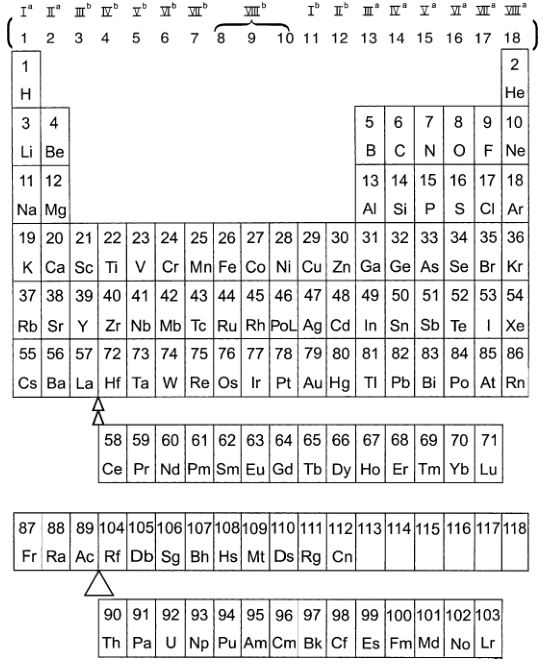
\includegraphics[clip,width=10cm]{8_1.JPG}
  \caption{元素周期表.将来104-110の元素は名前が変更されるか発見されるかするだろう.}
  \label{table8.1}
\end{figure}

周期表の下に行くにつれ、バンドギャップの幅が減少するという一般的な傾向をすでに目にしている。SiCは$\mathrm{I\hspace{-1pt}V}$属の半導体に所属する。SiCは、複数の異なるポリタイプを形成するので悪名高い。それらすべての間接的なバンドギャップはおおよそ3 eVで、ダイヤモンドとSiのギャップの間である。

炭素は、グラファイトやグラフェン[09N1]、ナノチューブ、そしてフラーレン($\mathrm{C_{60}}$)といったさらなる変形[08S1]を持つ。グラファイトは、六角形の層と層間の弱いファンデルワールス結合の中に、より強い共有$sp^2$混成軌道をもつ半金属である。$\mathrm{C_{60}}$は$E_{\mathrm{g}}\approx2.2 \mathrm{eV}$の半導体である。グラフェンとナノチューブは半導体にも、半金属にも、金属にもなれる。

ダイヤモンド型構造において、全ての原子は、最近接原子によって四面体に囲まれている。図7.2を見ること。例えばGe原子のある副格子をGa(外殻電子が1つ不足している)に、もう一つをAs(外殻電子がGeより1つ多い)に置き換えることができ、このとき単位格子ごとの電子の総量は変化しておらず、ほんの少しのイオン結合が加わっているが、まだ共有結合が支配的である。この手順では、点群$T_d$で$\mathrm{I\hspace{-1pt}I\hspace{-1pt}I-V}$の閃亜鉛鉱型結晶構造と呼ばれるものが導かれる。この半導体の集団は、B,Al,Ga,InとN,P,As,Sbの化合物である。BNは絶縁体、AlN,GaNは広いギャップを持つ半導体、InSbは狭いバンドギャップを持つ半導体であるという、周期表におけるバンドギャップの一般的な傾向が見られる。


$\mathrm{I\hspace{-1pt}I\hspace{-1pt}I}$群の窒化物は六角形のウルツ鉱型結晶構造(点群$C_{6V}$)として優先的に結晶化される。この場合、片方の種類のすべての原子は、もう片方の原子に四面体に囲まれているが、2番目に近い原子の配置は、六角形構造が展開するようなものである(図7.2参照)。

もしこの手順を、$\mathrm{I\hspace{-1pt}V}$半導体から$\mathrm{I\hspace{-1pt}I\hspace{-1pt}I-V}$化合物が導けたように、もう1度か2度繰り返した場合、イオン結合が増加し、最終的に支配的となるが、しかしまだ一般的な四面体配置である、$\mathrm{I\hspace{-1pt}I-V\hspace{-1pt}I}$(正確には$\mathrm{I\hspace{-1pt}I^B-V\hspace{-1pt}I^A}$)や%見づらいから改行
$\mathrm{I-V\hspace{-1pt}I\hspace{-1pt}I}$(正確には$\mathrm{I^B-V\hspace{-1pt}I\hspace{-1pt}I^A}$)半導体が得られる。$\mathrm{I\hspace{-1pt}I^A-V\hspace{-1pt}I^A}$や$\mathrm{I^A-V\hspace{-1pt}I\hspace{-1pt}I^A}$化合物は普通絶縁体で、岩塩構造やCsCl構造で結晶化される。

\renewcommand{\figurename}{表}%図表記をFigure *.*へ
\setcounter{figure}{1}
\begin{figure}[htb]
  \centering
  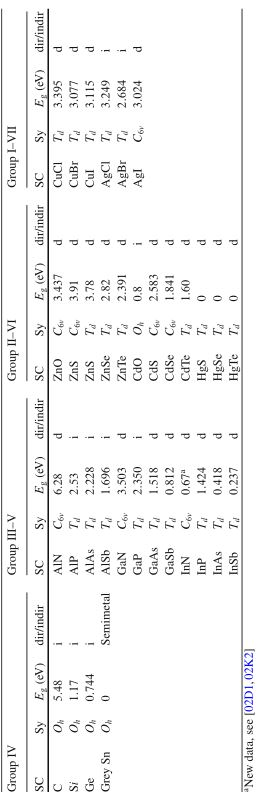
\includegraphics[clip,height=16cm]{8_2.JPG}
  \caption{低温($T\lesssim10\,K$)における$\mathrm{I\hspace{-1pt}V},\mathrm{I\hspace{-1pt}I\hspace{-1pt}I-V},\mathrm{I\hspace{-1pt}I-V\hspace{-1pt}I},\mathrm{I-V\hspace{-1pt}I\hspace{-1pt}I}$族半導体(SC)のバンドギャップエネルギーの値.Sy:Symmtry(点群).第1章[82L1]及び[01V1,04A1]による.}
  \label{table8.2}
\end{figure}

$\mathrm{I\hspace{-1pt}I-V\hspace{-1pt}I}$半導体はZn,Cd,HgとO,S,Se,Teを含む化合物である。ZnS,ZnO,CdSは広いギャップの半導体であるが、水銀化合物はふつう半金属であるように、周期表の下に行くにつれ、一般的にギャップはまた減少する。$\mathrm{I\hspace{-1pt}I-V\hspace{-1pt}I}$半導体は、少数の例外を除きふつう閃亜鉛鉱型かウルツ鉱型で結晶化される。両方の構造は一部、わずかなエネルギーの違いだけで可能である。例えば、これはZnSの場合である。

CdO(岩塩構造)やHgO(菱面体)のように、いくつかの化合物はほかの構造をとれる。HgSは閃亜鉛鉱型構造をとる場合は半金属だが、三方晶系(cinnabar:辰砂)をとる場合は、約2.2 eVのギャップを持つ半導体である。

主な$\mathrm{I-V\hspace{-1pt}I\hspace{-1pt}I}$化合物は表8.2に記載されている。最も調査されているものは、フッ化物を除くCuハロゲン化物やAgハロゲン化物である。フッ化物や$\mathrm{Ag^+}$ハロゲン化物の半導体としての性質についてはあまり知られていない。

今まで、本文では元素や二元化合物のみを含んでいた。上と同じような方法で、$\mathrm{CuGaSe_2}$のような三元半導体や、$\mathrm{Ag_2CdGeS_4}$のような四元半導体でさえ得られる。

さらに、いくつかの元素や多くの二元化合物は、$\mathrm{Si}_{1-x}\mathrm{Ge}_{x}$,$\mathrm{Ga}_{1-y}\mathrm{Al}_{y}\mathrm{As}$,$\mathrm{Cd}\mathrm{S}_{1-x}\mathrm{Se}_{x}$,$\mathrm{Zn}\mathrm{Se}_{1-x}\mathrm{Te}_{x}$,
$\mathrm{Cd}_{1-y}\mathrm{Hg}_{x}\mathrm{Te}$など、ギャップの混和性なしに、一部合金の形をとる。合金中では、原則として、一つは周期格子構造をもつ良い結晶だが、一つの副格子の格子点が、2つの異なる原子($\mathrm{Si}_{1-x}\mathrm{Ge}_{x}$)、陰イオン($\mathrm{Cd}\mathrm{S}_{1-x}\mathrm{Se}_{x}$)、陽イオン($\mathrm{Ga}_{1-y}\mathrm{Al}_{x}\mathrm{As}$)にランダムに占められている。
しかし、微視的にみると、組成$x$の濃度の揺らぎは何らかの障害として紹介される。

いくつかの合金は、CuPt構造という呼び名が採用されている、$\mathrm{Ga}_{0.5}\mathrm{In}_{0.5}\mathrm{P}$のような、組成が0.5に近い秩序構造を形どる傾向がある。

合金化は、$\mathrm{Ga}_{1-y}\mathrm{Al}_{y}\mathrm{N}_{x}\mathrm{As}_{1-x}$のように両方の副格子を持つことも可能である。

この本の残りの例のほとんどは、これらのより一般的な半導体からとられるが、さらにたくさんあり、そのうちのいくつかを下に述べる。

$\mathrm{I\hspace{-1pt}V-V\hspace{-1pt}I}$化合物(鉛塩として知られる)はPb,SnとS,Se,Teの化合物を含む。これらは一部IRレーザーダイオードとなる。PbSeは0.3 eVの直接遷移型ギャップを持つ[07Z1]。

P,Iといった、S,Se,Teのような元素半導体がさらに存在する(As,Sbは半金属とみなされる)。$\mathrm{GeO_2}$,$\mathrm{SnO_2}$といった$\mathrm{I\hspace{-1pt}I^B}$酸化物($\mathrm{SiO_2}$は石英で、絶縁体である)のほかに、$\mathrm{CUO_2}$(13.2章参照)と$\mathrm{TiO_2}$およびこれらの様々な変形(鋭錐石:anatase、金紅石:rutile、板チタン石:brookite)や、高い毒性を有するTlハロゲン化物半導体としての酸化物が存在する。このセクションを終えるため、アントラセン(anthracene:$\mathrm{C_{14}H_{10}}$)、ペンタセン(pentacene:$\mathrm{C_{22}H_{14}}$)、%見づらいから改行
ジベンゾチオフェン(dibenzothiophene:$\mathrm{C_{12}H_{8}S}$)、ヘキサチオフェン(hexathiophene)の結晶のような有機半導体に注目する。この本において有機半導体は焦点にないが、時折、光学的性質についての例を与えてくれる。

半導体のギャップは、温度の上昇とともに減少していくという一般的な傾向がある。減少幅$\Delta E_{\rm{g}}(T)=E_{\rm{g}}(T=0)-E_{\rm{g}}(T)$は温度変化とともに、低い温度域($T\leq100\rm{K}$)では二次元的に、高い温度域では直線的に変化する傾向がある。この振る舞いはVashiniの公式[67V1]によってよく記述される。

\begin{equation}
  \Delta E_{\rm{g}}(T)=\frac{\alpha T^2}{\beta+\gamma T}
  \tag{8.8a}
\end{equation}
より複雑な公式が、たとえば[94A1,99P1,00L1,02G1,03g1,03S1,06H1]やそれらの参照の中で、最近提案された。[99P1]では、たとえば(8.8b)が与えられている。

\begin{equation}
  \Delta E_{\rm{g}}(T)=\frac{\alpha\theta_P}{2}\left[\sqrt[P]{1+\frac{2T}{\Theta_P}}-1\right]
  \tag{8.8b}
\end{equation}
ここで、$\Theta_P$は効果的なフォノン温度、$\alpha$はエントロピーの高温限界、$P$は物質固有の3番目のパラメータである。

バンドギャップは変形ポテンシャル(8.21)に依存するため、$\Delta E_{\rm{g}}(T)$、つまりキャリア-フォノン結合に対し、フォノン容積と格子定数の温度依存性の2つの大きな寄与がある。

CuClや鉛塩などのようないくつかの半導体は、温度の上昇とともに$E_\mathrm{g}$が増加し、CuBrのような別の半導体では、$E_\mathrm{g}(T)$は温度の上昇とともに最大値を通り過ぎる。たとえば[82L1]の第1章や、その参照の中にデータが載っている。

\subsection{新しい準粒子としての電子と正孔}

今後見るように、半導体の電子系の光学特性は、上の価電子帯と下の伝導帯の間の電子の遷移に大きく支配されている。

図8.1-8.5に関連して今まで述べられたバンド構造は、次の文で$N\pm1$粒子問題と呼ばれるものについて述べる。価電子帯が$1\,\mathrm{cm}^{-1}$当たり$N$個の電子で満たされていて、
\begin{equation}
  N\simeq10^{22}-10^{23}\,\mathrm{cm}^{-3}
  \tag{8.9}
\end{equation}
かつ伝導帯が完全に空である状態に、さらに1つ電子が加わった半導体を考えた時、電子は確かに伝導帯の状態に位置する。$N$この電子から1つ電子が取り除かれて、その電子がどこから来たのかを尋ねた時、その答えは価電子帯である。

今明らかな段階は、空の伝導帯(CB)中の1つか少しの電子を考えることである。ほとんど満たされた価電子帯においては、その逆で、たくさん占められている電子の代わりに、少しの空の状態やその特性を考えるほうがより簡単である。この考え方は、"欠陥電子"や"正孔"の概念を導く。正孔の特性は、価電子帯(VB)から取り除かれた電子の特性とともに次の方法(表8.3)につながる。

\setcounter{figure}{2}
\begin{figure}[b]
  \centering
  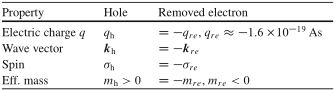
\includegraphics[clip,width=9cm]{8_3.JPG}
  \caption{正孔を作るために価電子帯から取り除かれた電子の性質と比べた価電子帯の正孔の性質.}
  \label{table8.3}
\end{figure}

表8.3から、正孔は正電荷を持ち、その波数ベクトルやスピンは、価電子帯から取り除かれた電子のそれと逆であることが分かる。価電子帯が完全に満たされた半導体は、合計の運動量やスピンはゼロに等しい。もし1つの粒子が取り出された場合、残りは、取り除かれた粒子と逆のthe above quantities valuesを得る。明確にするために、図8.6a,bは、伝導帯に1つの電子を、価電子帯に1つの正孔を含むバンド構造を示している。状態は$\bm{k}$(2.6章参照)においては等価で、しかし、それぞれのバンドには$\mathrm{cm}^3$当たりふつう$10^{22}-10^{23}$の状態があり、図8.6のように少数ではない。

半導体結晶の電子と正孔は準粒子である。これらは、普通の電子や陽電子のエネルギーギャップの大きさ($\simeq1\,\mathrm(MeV)$)、すなわち、$511\,\mathrm{keV}=m_0c^2$の残りの2倍の質量であることを除いて、一般にたくさんある普通の電子や陽電子とは対照的に、結晶の中にのみ存在でき、真空中には存在できない。電子と正孔の分散関係は、式(8.10)で与えられる、非相対論的な場合の自由電子や陽電子の分散関係とは異なる。
\begin{equation}
  E_{\mathrm{e,p}}=\pm\left(m_0c^2+\frac{\hbar^2k^2}{2m_0}\right)
  \tag{8.10}
\end{equation}
ここで、$m_0$は自由電子の質量である。

\renewcommand{\figurename}{図}%図表記をFigure *.*へ
\setcounter{figure}{5}
\begin{figure}[tb]
  \centering
  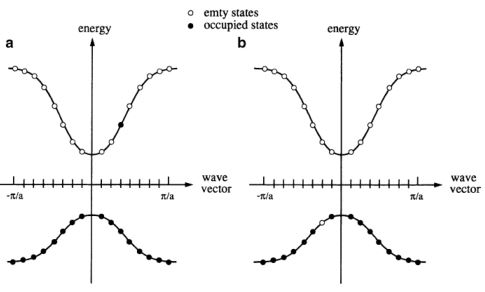
\includegraphics[clip,width=9cm]{8_6.JPG}
  \caption{$N\pm1$粒子問題を表している伝導帯における1つの電子(a)と価電子帯における1つの正孔(b).(黒点:占有状態、白点:空の状態)}
  \label{8.6}
\end{figure}

結晶電子や結晶正孔の量$\hbar\bm{k}_{\mathrm{e,p}}$は準運動量であり、逆格子ベクトルのmodで保存され(8.4や8.5を参照)、ブロッホ波(8.2、8.3)は運動量演算子$\frac{\hbar}{\mathrm{i}}\nabla$の固有値ではない。準運動量の概念のさらなる詳細は、5章の[98B1]を見ること。

価電子帯のより深くに存在する正孔のエネルギーは上昇する、ということに注意。



\end{document}
